\documentclass[8pt]{report}
\input{preamble}
\usepackage{arev}

\usetikzlibrary{positioning}
\title{\Huge{Devoir 1}\\{IFT1065C — Structures discrètes en informatique}}
\author{\huge{Aiya Ben Ouhida et Franz Girardin}}
\date{30 Septembre 2023}
\lstset{inputencoding=utf8/latin1}


\usepackage{graphicx}
\usepackage{caption}
\usepackage{subcaption}


\usepackage{balance}
\usepackage{mathpazo}
\usepackage{dirtree}
\usepackage{titlesec}
\titleformat{\chapter}
  {\small\bfseries} % format
  {}                % label
  {0pt}             % sep
  {\huge}           % before-code


\usepackage{lipsum}
\usepackage{titling}
\renewcommand\maketitlehooka{\null\mbox{}\vfill}
\renewcommand\maketitlehookd{\vfill\null}


\newcommand{\varitem}[3][black]{%
  \item[%
   \colorbox{#2}{\textcolor{#1}{\makebox(5.5,7){#3}}}%
  ]
}


\usepackage{afterpage}
\newcommand\myemptypage{
    \null
    \thispagestyle{empty}
    \addtocounter{page}{-1}
    \newpage
    }



\newcommand{\ClaudioList}{red,DarkOrange1,Goldenrod1,Green3,blue!50!cyan,DarkOrchid2}
\newcommand{\SebastianoItem}[1]{\foreach \X[count=\Y] in \ClaudioList
{\ifnum\Y=#1\relax
\xdef\SebastianoColor{\X}
\fi
}
\tikz[baseline=(SebastianoItem.base),remember
picture]{%
\node[fill=\SebastianoColor,inner sep=4pt,font=\sffamily,fill opacity=0.5] (SebastianoItem){#1)};}
}
\newcommand{\SebastianoHighlight}{\tikz[overlay,remember picture]{%
\fill[\SebastianoColor,fill opacity=0.5] ([yshift=4pt,xshift=-\pgflinewidth]SebastianoItem.east) -- ++(4pt,-4pt)
-- ++(-4pt,-4pt) -- cycle;
}}    
%====================================================================

%====================================================================
\newcommand*{\authorimg}[1]%
    { \raisebox{-1\baselineskip}{\includegraphics[width=\imagesize]{#1}}}
\newlength\imagesize  




\begin{document}


\maketitle
\pagebreak
\tableofcontents
\pagebreak
\chapter{Problèmes du devoir 1}
\section*{\textnormal{PROBLÈME 1.1 \;\;\;\; $\cdot$ \;\;\;\; INFINIEMENT VIDE \hspace*{\fill} (\textit{30 points})}}


\noindent Les règles du problème ne permettent pas de placer d'objet à l'intérieur d'un ensemble. 
Or, l'utilisation de l'ensemble vide comme point de départ ne semble pas être prohibée par ces mêmes règles.
    Pour débuter la construction de notre ensemble, posons alors : 
    \begin{align}
        A = A_0 = \emptyset \label{eq:AEmptySetEq}
    \end{align}
    Une des opérations autorisées, soit \textbf{l'ensemble puissance}, nous permettra 
    d'élaborer la construction de notre ensemble. 
    \begin{enumerate}
        \item En applicant l'opération d'\textbf{ensemble puissance} sur $A$ on obtient un ensemble qui contient 
            \textit{tous les sous-ensembles possibles} de $A$. Puisque l'ensemble vide est un sous-ensemble de 
            tous les ensembles (y compris lui-même) et puisqu'il n'y a pas d'autre ensemble 
            pouvant être un sous-ensemble de l'ensemble vide auquel nous avons assigné la variable $A$ dans 
            ce cas-ci, nous avons : 
            \begin{align}
                \label{eq:A_1}
                \mathcal{P}(A) = \mathcal{P}(\emptyset) = \{ \emptyset \} = A_1       
            \end{align}
    \end{enumerate}
    \begin{note}{}{}
        Pour s'assurer que $\emptyset$ est \textbf{l'unique sous-ensemble possible} en appliquant $\mathcal{P}(A)$,
        nous utilisons la propriété selon laquelle le cardinal de l'ensemble puissance est égale
        à $2$ exposant le cardinal de l'ensemble d'origine : 
        \[ |\mathcal{P}(A)| = 2^{|A|} = 2^0 = 1 \]
    \end{note}

    \begin{enumerate}
        \setcounter{enumi}{1}
        \item Puisque l'ensemble ainsi formé est différent de l'ensemble vide, nous venons de construire, 
            en utilisant une opération ensembliste et sans supposer l'existance préalable d'un objet, 
            un ensemble autre autre que l'ensemble vide. 
    \end{enumerate}

    
    \begin{Reponse}{}{}
                \[ \mathcal{P}(\emptyset) = \{ \emptyset \} \neq \emptyset \implies A_0 \neq A_1\] 
    \end{Reponse}



\section*{\textnormal{PROBLÈME 1.2 \;\;\;\; $\cdot$ \;\;\;\; INFINIEMENT VIDE }}   
    \noindent Grâce au problème 1.1, nous savons qu'il est possible de construire un ensemble distinct à 
    partir de l'ensemble vide. Nous constatons également que le cardinal de ce nouvel ensemble est 
    supérieur au cardinal de l'ensemble vide—soit l'ensemble d'origine. \\\\ 
    Nous nous servirons de ces observations pour construire une série d'ensembles tous distincts les uns des 
    autres tel que chaque nouvel ensemble contient un plus grand nombre d'éléments que son précédesseur. 
    \begin{enumerate}
        \item Notons que l'application de l'opération d'ensemble puissance sur le résultat de l'équation  
        \eqref{eq:A_1} engendre un nouvel ensemble distinct de $A_1$. 
        \begin{align}
            \label{eq:EmptysetA_2}
        \mathcal{P}(A_1) = \mathcal{P}(\{ \emptyset \}) = 
        \{ \emptyset, \{ \emptyset \} \} = A_2 \neq A_1 
        \end{align}

       \item Nous pouvons répéter l'opération sur $A_2$ pour obetenir $A_3$ :
        \begin{align}
            \label{eq:EmptysetA_3}
            \mathcal{P}(A_2) = 
            \mathcal{P}(\{ \emptyset, \{ \emptyset \}\}) = 
            \{ \emptyset, \{ \emptyset \}, \{\{ \emptyset \}\}, \{\emptyset, \{\emptyset\}  \} \} = 
            A_3 \neq A_2 
        \end{align}
    \end{enumerate}
    \begin{note}{}{}
        Nous mettons en évidence la démarche des équations \eqref{eq:EmptysetA_2} et \eqref{eq:EmptysetA_3} 
        pour expliciter l'intuition suivante : l'application de l'opération d'ensemble puissance sur un 
        ensemble donné \textbf{engendre un unsemble qui peut être à son tour utilisé pour rappliquer 
        cette opération ensembliste}. 
        Ce processus peut être répété à pertétuité pour générer \textit{une infinité d'ensembles} 
        tous distincts l'un de l'autre et dont le cardinal croît exponentiellement. 
    \end{note}
    \begin{enumerate}
        \setcounter{enumi}{2}
        \item Nous pouvons donc générer \textbf{une suite infinie d'ensembles disctincts} 
            à partir de l'opération d'ensemble puissance, sans supposer l'existance préalable d'un objet :
    \end{enumerate}


    \begin{Reponse}{}{}
            Selon, les équations (1.1) à (1.4), la formule suivante permet de générer une infinité d'ensemble. 
            \begin{align*}
                A_1 = \emptyset, A_n = \mathcal{P}(A_{n-1}) \;\; \forall n \geq 2. 
            \end{align*}
    \end{Reponse}


\section*{\textnormal{PROBLÈME 1.3 \;\;\;\; $\cdot$ \;\;\;\; INFINIEMENT VIDE }}  

    Nous allons montrer que la notation du mathématicien polonais 
    $Kazimierz \; Kuratowski^1$ pour représenter une paire ordonnée est valide. 
    Selon cette notation, il est possible de représenter une paire ordonnée $P$ par un ensemble $A$ de cardinal 
    $|A| = 2$ où le 
    premier élément de $A$ est un singleton contenant la première entrée de la paire, et le second élément de $A$ 
    est un ensemble contenant uniquement le premier élément et le second élément de la paire : 
    \[ P = (a, b) = \Bigl\{ \{ a \}, \{a, b \}  \Bigr\} \]  

    De façon informelle, nous pouvons dire que le fait que $a$ apparaisse seul dans un ensemble, puis qu'il apparaisse 
    à nouveau dans un ensemble contenant également $b$ permet de 
    \textit{marquer l'ordre de a par rapport à b dans la paire ordonnée}. 
    Plus formellement, la notation de Kuratowski repose sur deux axiomes :
    \begin{enumerate}
        \item La \textit{propritété} d'appartenir \textbf{aux deux ensembles} contenus dans 
            $A$ est associée à la propriété d'être la première entrée de la paire ordonnée. 

        \item La \textit{propriété} d'appartenir à \textbf{un seul des ensembles} contenus dans $A$ est 
            associée à la propriété d'être la seconde entrée de la paire ordonnée. 
    \end{enumerate}
    En considérant ces deux axiomes, la notation de Kuratowski est valide. En effet, elle est valide précisément parce  
    qu'elle respecte \textit{le principe d'indentité} d'une paire ordonnée. Ce qu'on conçoit comme étant une paire 
    ordonnée dépend du principe d'identité :
    \textit{une paire ordonnée $P$ est identique à une paire ordonée $Q$ si et seulement si l'élément de la première 
    paire à une position donnée est indentique à l'élément de la secondaire paire à cette même position}. 
    \[  P = (a,b) = Q = (c,d) \Leftrightarrow  \;a = c, \;\;b = d \] 

    Le corollaire de ce principe est que si $a$ est différent de $c$ et $b$ est différent de $d$, les paires 
    $P$ et $Q$ sont nécessairement différentes : 
    \[ a \neq c, b \neq d, a \neq b \implies P \neq Q   \]
    Si la notation de Kuratowski est valide, la représentation 
    de $P = (a, b)$ et la représentation de $Q = (c, d)$ devraient engendrer des ensembles différents. 
    \[  P = (a, b) = \Bigl\{ \{ a \}, \{a, b \}  \Bigr\} \neq \Bigl\{ \{ c \}, \{c, d \}  \Bigr\} = (c, d) = Q\;\; 
    \Big| \;\; a \neq c, \;\; b \neq d  \]
    Notons que l'inéquivalence $P \neq Q$ est une conséquence directe du principe d'identité appiqué aux ensembles : 
    deux ensembles sont identiques si et seulement si ces ensembles contiennent les même éléments. Par ailleurs,
    les paires $(a, b)$ et $(c, d)$ sont identiques uniquement lorsque tous les éléments $a, b, c, d$ sont identiques : 
    \[ P = (a, b) = (b, a) \implies a = b \;\; (\textit{Paire ordonnée}  )  \] 
    \[ P =  \Bigl\{ \{ a \}, \{a, b \}\Bigr\} =  \Bigl\{ \{ b\}, \{b, a \}\Bigr\} \implies a = b \;\; (Kuratowski) \]
    \begin{align*}
         P = (a, b) = (b, a) = (c, d) = (d, c) \\
         = \Bigl\{ \{ a \}, \{a, b \}\Bigr\} =  \Bigl\{ \{ b\}, \{b, a \}\Bigr\} \\
         = \Bigl\{ \{ c \}, \{c, d \}\Bigr\} =  \Bigl\{ \{ d\}, \{d, c \}\Bigr\}  \\
         = Q \implies a = b = c = d        
    \end{align*}
    La notation de  
    Kuratowski engendre donc des ensembles différents pour des paires ordonées qui sont différents. Conversement, 
    elle engendre des ensembles identiques pour des paires ordonnées qui sont identiques. 
    \begin{Reponse}{}{}
        Grâce à la \textbf{notation de Kuratowski}, 
        il est possible de représenter une paire $(a,b)$ sous forme d'un ensemble,
        de sorte qu’il soit possible de retrouver sans ambiguïté l’ordre des éléments de la paire. 
    \end{Reponse}




\section*{\textnormal{PROBLÈME 1.1 \;\;\;\; $\cdot$ \;\;\;\; LISTES UNIVERSELLES \hspace*{\fill} (\textit{30 points})}}. 

\noindent Nous savons que les listes possibles sur \textbf{1 bit} est l'ensemble $A$ de listes de un élément 
              tel que cet élément appartient à l'ensemble des deux entités binaires possibles :
              \[ A = \Bigl\{ (a) \;\; | \;\; a \in \{0,1\} \Bigr\} \]
              \begin{Reponse}{}{}
                  Les seuls listes possibles sur $1$ bit sont donc $(0)$ et $(1)$. Par ailleurs, \textbf{la liste} 
                  $L_1 = (0,1)$ est une \textit{liste universelle} sur 1 bit : 
                  \\\\ Soit $0 \in (0) \text{ et } 1 \in (1)$,
                  \begin{center} 
                      $0 \in (0, 1), \; 1 \in (0,1) \Leftrightarrow (0) \text{ et } (1) 
                      \text{ sont des sous-listes de } L_1$ 
                      \\ 
                      $\Updownarrow$  
                      \\ 
                      $L_1$ est une liste universelle sur $1$ bit.  
                  \end{center}
              \end{Reponse}
              \section*{\textnormal{PROBLÈME 1.2 \;\;\;\; $\cdot$ \;\;\;\; LISTES UNIVERSELLES}} 

              \noindent Nous savons que les listes possibles sur \textbf{2 bits} est représenté par  
              $A_2$, l'ensemble des listes de deux éléments telles que ces éléments appartiennent 
               à l'ensemble des deux entités binaires possibles. 
            \begin{center}
                    $ A_2 = \{ (a,b) \;\; | \;\; a, b \in \{0, 1\} \}$ \\
            \end{center}

            \begin{Reponse}{}{}
                Les seules listes possibles sur \textbf{2  bits} sont donc $l_1 = (0,0), l_2 = (0, 1), l_3 = (1, 0)$ et 
                $l_4 = (1,1)$ Par ailleurs, la \textbf{liste} $L_2 = (0, 0, 1, 1)$ est une  
                liste universelle sur 2 bits.  
            \end{Reponse}

 

            \begin{figure}[H]
            \begin{center}
            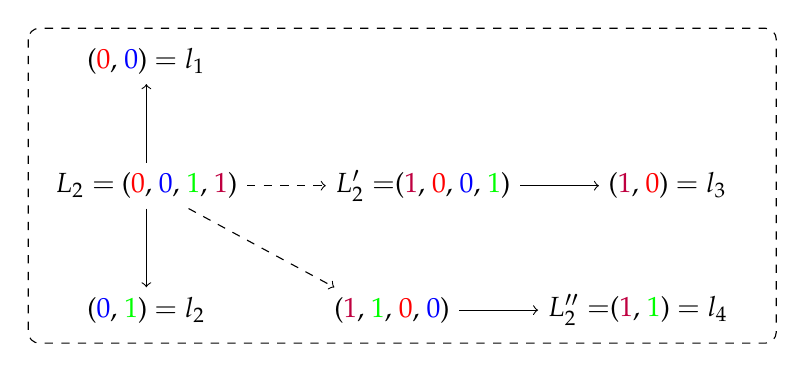
\begin{tikzpicture}[node distance=1cm]
              % Les éléments de la liste
                \node (0011) {$L_2 =$ (\textcolor{red}{0}, \textcolor{blue}{0}, \textcolor{green}{1}, \textcolor{purple}{1})};
                \node[above=of 0011] (00) {(\textcolor{red}{0}, \textcolor{blue}{0}) $= l_1$};
                \node[below=of 0011] (01) {(\textcolor{blue}{0}, \textcolor{green}{1}) $= l_2$};
                \node[right=of 0011] (1001) {$L_2^{\prime} = $(\textcolor{purple}{1}, \textcolor{red}{0}, \textcolor{blue}{0}, \textcolor{green}{1})};
                \node[right=of 01] (1100) {\;\;\;\;(\textcolor{purple}{1}, \textcolor{green}{1}, \textcolor{red}{0}, \textcolor{blue}{0})};

                \node[right=of 1001] (10) {(\textcolor{purple}{1}, \textcolor{red}{0}) $= l_3$};
                \node[right=of 1100] (11) {$L_2^{\prime\prime} = $(\textcolor{purple}{1}, \textcolor{green}{1}) $= l_4$};
              
              % Encadrement de la liste universelle
              \draw[dashed, rounded corners] (-1.5,2) rectangle (8,-2);
              
              % Flèches pour montrer les sous-ensembles circulaires
              \draw[->] (0011) -- (00);
              \draw[dashed,->] (0011) -- (1001);
              \draw[dashed,->] (0011) -- (1100);
              \draw[->] (0011) -- (01); 
              \draw[->] (1001) -- (10);
              \draw[->] (1100) -- (11);
            \end{tikzpicture}
            \end{center}
            \caption{Rotations de $L_2$ permettant d'obtenir $l_1, l_2, l_3, l_4$ (TikZ).}
            \end{figure}


\section*{\textnormal{PROBLÈME 1.3 \;\;\;\; $\cdot$ \;\;\;\; LISTES UNIVERSELLES}}.

                \noindent Nous savons que les listes possibles sur \textbf{3 bits} est représenté par 
                $A_3$, 
                    l’ensemble des listes de trois éléments telles que ces éléments appartiennent 
                    à l’ensemble des deux entités binaires possibles. 

            \begin{center}
                    $ A_3 = \{ (a,b, c) \;\; | \;\; a, b, c \in \{0, 1\} \}$ \\
            \end{center} 


            \begin{Reponse}{}{}
                Les seules listes possibles sur \textbf{3  bits} sont donc 
                $l_5 = (0,0,0),\; l_6 = (0,0,1),\; l_7 = (0, 1, 0),\; l_8 = (0,1,1),\; l_9 = (1,0,0),\; 
                l_{10} = (1,0,1), \; l_{11} = (1,1,0), \; l_{12} = (1,1,1)$. \\ 
                Par ailleurs, la \textbf{liste} $L_3 = (1, 1, 1, 0, 0, 0, 1, 0)$ est une liste 
                universelle sur 3 bits.  
            \end{Reponse}

\section*{\textnormal{PROBLÈME 1.4 \;\;\;\; $\cdot$ \;\;\;\; LISTES UNIVERSELLES}}.
        \begin{Reponse}{}{}
            Il n'est pas possible de construire une liste universelle sur 3 bits ayant moins de $2^3 = 8$ 
            éléments.
        \end{Reponse}
        Nous partons du principe 
        $P_1$ selon lequel, 
        pour obtenir une liste universelle $L$ sur $n$ bits, la liste doit contenir au moins 
        $2^n$ éléments. Nous allons prouver, par l'absurde, que cette proposition est vraie. \\\\  

        Supposons la négtion de la proposiion, soit $\neg P_1 = P_1^{\prime}$. 
        Autrement dit, supposons qu'\textit{une liste universelle sur 
        $n$ bits peut contenir \textbf{moins de $2^n$} éléments} (\textit{proposition} $P_1^{\prime}$).  
        \\\\ 
        Considérons le scénarios le plus simple. Le nombre de bit non-nul et non négatif le 
        plus petit pouvant être considéré 
        est \textbf{1 bit}. Les listes possibles sur $1$ bit sont soit $l_1= (0)$ ou $l_2 = (1)$.Or, 
        selon $P_1^{\prime}$, il serait possible 
        qu'\textit{une liste universelle pour n = 1 bit contienne moins de $2^1$ = $2$ éléments}. 
        Les seules listes (naturelles) 
        de moins deux éléments pouvant être considérées—comme liste universelle potentielles sur $1$ bit—
        sont les listes $(0)$ ou $(1)$. 
        \\\\
        Or, ni $(0)$ ni $(1)$ n'est une liste universelle sur 
        $1$ bit, puisqu'aucune de rotation $(0)$ ne permet d'obtenir à la fois $(0)$ et $(1)$; et aucune rotation 
        de $(1)$ ne permet d'obtenir à la fois $(0)$ et $(1)$. 
        \begin{enumerate}
            \item Affirmer que $(0)$ est une liste universelle sur 1 bit est une contradiction de la définition 
                d'une liste universelle. 
            \item Affirmer que $(1)$ est une liste universelle sur 1 bit est une contradiction de la définition 
                d'une liste universelle. 
 
            \item Par contre-exemple, on a montré que $P_1^{\prime}$ mène à une contradiction.
            \item Par conséquent, nous avons : 
                \[ (\neg P_1 \implies Faux) \implies P_1 \equiv (P_1^{\prime} \implies Faux) \implies P_1 \]     
        \end{enumerate}
        Ainsi, $P_1$ est vraie. 


\section*{\textnormal{PROBLÈME 3.1 \;\;\;\; $\cdot$ \;\;\;\; JEU DU 10 \hspace*{\fill} (\textit{30 points})}} 

        \noindent L'énoncé indique qu'on cherche à trouver la probabilité qu'un évènement, $C$, se produise 
        sachant qu'un évènement $B$ s'est déjà produit. Pour déterminer cette probabilité, nous allons utiliser 
        le principe de \textit{probabilité conditionnelle}. Soit les évènements suivants : 
        \begin{enumerate}
            \varitem{blue!40}{\textcolor{white}{$C$}} l'évènement où la première carte est $A, K, Q$ ou $J$ 
            \varitem{blue!40}{\textcolor{white}{$B$}} l'évènement où la première carte est $A, 10$ ou $5$
            \varitem{blue!40}{\textcolor{white}{$C^{\prime}$}} l'évènement où la première carte est $A$
        \end{enumerate}

        \vspace{1em}
        \noindent Nous déduison $C^{\prime}$ de $B$ et $C$, puisque la première carte peut seulement être un $A$, si 
        elle est contraintes à être $A, 10$ ou $5$, sachant qu'elle est $A, K, Q$ ou $J$. Nous avons : 


        \begin{enumerate}
            \varitem{blue!40}{\textcolor{white}{$1$}} $P(B^{\prime}|C)$ la probabilité de $B^{\prime}$ 
            sachant que C s'est produit 
            \varitem{blue!40}{\textcolor{white}{$2$}} $P(B^{\prime}\cap C)$ la probabilité que $B^{\prime}$ 
            et $C$ se produisent.
            \varitem{blue!40}{\textcolor{white}{$3$}} $P(B^{\prime})$ la probabilité que $B^{\prime}$ se produise. 
        \end{enumerate} 
        \vspace{1em}
        \noindent Calculons alors les probabilités que chaque évènements se produisent : 
        \begin{enumerate}
            \item $P(C)$ = $\dfrac{4 \text{ valeurs} \times 4 \text{ sortes}}{40 \text{ cartes total}} = 
                \dfrac{16}{40} = \dfrac{2}{5}$
            \item $P( B^{\prime} \cap C) = P(B^{\prime})$; la probabilité que la première carte soit $A$ et, 
                \textbf{à la fois}, $A, K, Q$ ou $J$ est simplement la probabilité qu'elle soit $A$. Autrement dit, 
                on considère pas la probabilité qu'elle puisse être $A$ et $K$; ni $A$ et $Q$; ni $A$ et $J$. On peut 
                seulement considérer la probabilité qu'elle soit $A$ et $A$, \textbf{à la fois}.
            \item $P(B^{\prime}) = \dfrac{4 \text{ cartes de valeur \textit{A}}}{40 \text{ cartes total}} 
                = \dfrac{4}{40} = \dfrac{1}{10}$
            \item $P(B^{\prime}|C) = \dfrac{P(A\cap B)}{P(C)} = \dfrac{\frac{1}{10}}{\frac{2}{5}} = \dfrac{1}{4}$
        \end{enumerate}

        \begin{Reponse}{}{}
            La probabilité conditionnelle que la première carte soit de valeur $A$, sachant qu'elle est de valeur $A, K, Q$ ou $J$ 
            est logiquement équivalente à la probabilité conditionnelle que la première carte soit de valeur  $A, 10$ ou $5$, sachant
            qu'elle est de valeur $A, K, Q$ ou $J$. Cette probabilité est \textit{une chance sur quatre}. 
            \[ P(B|C) = P(B^{\prime}| C) = \dfrac{1}{4} \]
        \end{Reponse}

        \section*{\textnormal{PROBLÈME 3.2 \;\;\;\; $\cdot$ \;\;\;\; JEU DU 10 }} 
        \noindent \textcolor{myb}{\textit{Scénario idéal}}\\ 
        \indent Considérons le premier joueur à qui nous distribuons une carte, selon l'ordre de distribution établit. Nous 
        savons qu'après un tour de distribution, $j_1$ aura une carte dont le type est parmis les types disponibles 
        $\{\spadesuit, \clubsuit, \diamondsuit, \heartsuit\}$. Nous savons également qu'un tour de distribution 
        correspond à $4$ \textbf{cartes distribuées}. Or, au $2^e$ tour de distribution $j_1$ pourrait avoir la chance 
        d'obtenir une autre carte du même type que le type de la carte qu'il a obtenu au premier tour. Si on s'arrête à 
        ce moment précis, il y aura \textbf{5 cartes ditribuées} et un joueur ayant au moins deux cartes du même type. 
        Cette situation correspond au scénario idéal. Nous savons donc que la solution réelle est supérieure à $N = 5 \; cartes$.

        \vspace{1em}
        \noindent\textcolor{myb}{\textit{Scénario pire des cas}}\\ 
        \indent Considérons le pire des cas possibles. Il s'agit d'un cas où, à chaque tour de distribution, 
        le $j_1$ obtient des cartes 
        de différents types. Ainsi, au $3^\text{e}$ tour, il possédera $3$ cartes de $3$ types différents et un total de $12$ 
        cartes aura été distribué. Au $4^\text{e}$ tour, dans le pire des cas, il aura nécessairement $4$ cartes de $4$ types 
        différents et $16$ cartes auront été distribué. \\\\ 
        \indent Or, au $5^\text{e}$ tour de distribution, la carte distribuée devra nécessairement être du même type que le type 
        d'une des cartes qu'il possède déjà. Nous évoquons le principe du pigeonnier. \\\\
        \indent En effet, si la main du $j_1$ 
        présente $k$ cases de types de cartes et que chacune de ces cases est déjà pleine, si on essait d'ajouter à sa 
        main une carte d'un des types possibles, sa nouvelle main contiendra $n > k$ cartes où au moins une case aura 
        deux cartes du même type. À ce moment précis, c'est-à-dire à la première carte distribuée du $5^{\text{e}}$ 
        tour, nous serons certain qu'au moins un joueur aura deux cartes du même type.
        \begin{Reponse}{}{}
            Il faut distribuer \textbf{$17$ cartes} pour être certain qu'au moins un des joueurs ait deux cartes du même type. 
        \end{Reponse}

        \section*{\textnormal{PROBLÈME 3.3 \;\;\;\; $\cdot$ \;\;\;\; JEU DU 10 }} 

        \noindent \textcolor{myb}{\textit{Modéliser la main de chaque joueur}}\\ 
        \indent Puisque l'ordre des carte n'est pas important, on peu utiliser un ensemble pour représenter la main 
        d'un joueur. Les objets qu'on place dans cet ensemble doivent être uniques. Une carte ne peut pas se trouver 
        dans la main de deux joueur à la fois. Il faut donc une représentation qui encapsule à la fois la valeur de la 
        carte et le type de la carte. On peut donc utiliser les symboles parmi  
        $\{\spadesuit, \clubsuit, \diamondsuit, \heartsuit\}$ combiné au valeurs possibles parmi les valeurs 
        $\{A, K, Q, J, 10, 9, 8, 7, 6, 5 \}$. Ainsi, la carte $10$ de coeur serait représenté par l'objet $10^\heartsuit$. 
        Par ailleurs, la main d'un joueur pourrait être représentée de la façon suivante : 
        \[ \{A^\heartsuit, K^\heartsuit, Q^\heartsuit, J^\heartsuit, 10^\heartsuit, 9^\heartsuit, 8^\heartsuit, 7^\heartsuit, 6^\heartsuit, 5^\heartsuit \} \]

        \noindent \textcolor{myb}{\textit{Modéliser l'ensemble du jeu}} \\
        \indent Puisque le jeu 10 nécessite que chaque joueur se place devant son cooéquipier, nous pouvons choisir une 
        structure discrète qui simule un ordre de main des joueurs. La \textbf{liste} semble être un choix approprié.

    En résumé, chaque main est un ensemble de cartes uniques, où chaque carte est représentée par une combinaison de sa valeur et de son type, par exemple, \[ \{A^\spadesuit, 10^\heartsuit, 6^\clubsuit, 7^\diamondsuit, \ldots\} \] Et la configuration totale du jeu est représentée par une liste de ces ensembles, par exemple, \[ \Big(\{A^\spadesuit, 10^\heartsuit, \ldots\}, \{K^\spadesuit, Q^\heartsuit, \ldots\}, \{J^\spadesuit, 9^\heartsuit, \ldots\}, \{7^\spadesuit, 8^\heartsuit, \ldots\}\Big) \].
        
        \begin{Reponse}{}{}
        Ainsi, la configuration d'un jeu de 10 peut être représentée par une liste contenant $4$ ensembles où chaque 
        ensemble représente la main d'un joueur et contient des objets uniques.       
        \end{Reponse}


        \section*{\textnormal{PROBLÈME 3.4 \;\;\;\; $\cdot$ \;\;\;\; JEU DU 10 }} 
        \noindent{\textcolor{myb}{\textit{Trouver les combinaisons possibles}}} 
        \indent D'après le modèle chosit, nous avons quatre ensembles distincts, chacun représentant la main 
        d'un joueur. Nous référerons à ces ensembles des comme s'il s'agissait de  \textbf{boîtes}. Nous avons \textbf{40} cartes à distribuer 
        et nous voulons trouver le nombre de combinaisons possibles. La \textit{loi multinomiale} permet de trouver 
        le nombre de façon différentes de distribuer $n$ objets dans $k$ \textbf{boîtes} différentes avec un nombre  
        spécifique $n_i \to n_k$ d'objets dans chaque boîtes: 
        \[ \dfrac{n!}{n_1!\cdot n_2!\cdot\ldots\cdot n_k!} \]
        Dans le contexte du problème, nous avons $n = 40$ \textbf{cartes}  et chaque \textbf{boîte}  a $10$ 
        objets et donc $n_1 = n_2 = n_3 = n_4 = 10$. Le nombre de façon différente d'arranger les cartes dans les 
        ensembles est donné par : 
        \[ \dfrac{40!}{10!\cdot10!\cdot10!\cdot10!} \] 
        \noindent{\textcolor{myb}{\textit{Trouver les configurations possibles}}}\\
        Or, nous avons choisit de placer les ensembles dans une liste. L'ordre de ces combinaisons est donc important. 
        Il y a $4!$ façons différentes d'organiser $4$ boîtes (ou les 4 ensembles) dans un ordre donné.

        \begin{Reponse}{}{}
        Le nombre de configurations 
        possibles, selon les structures discrètes choisi pour représenter le jeu, est donné par : 
        \[ 4! \cdot \dfrac{40!}{10!^4} \] 
        \end{Reponse}
        \section*{\textnormal{PROBLÈME 3.6 \;\;\;\; $\cdot$ \;\;\;\; JEU DU 10 }} 
        \indent Nous savons que chque joueur possède dix cartes en main, à la fin du processus de distribution. 
        Considérons alors $R$, le nombre de façons de choisir $10$ cartes parmi les $40$ du paquet : 
        \[  R = {40 \choose 10} \] 
        \indent Nous avons ${40 \choose 10}$ représentant le nombre de sous-ensembles possibles en choissisant $k = 10$ 
        éléments dans un ensemble de $40$ objets. Parmi ces ${40 \choose 10}$ sous-ensembles, plusieurs contiennent 
        $4$ as.         
        
        Pour mieux conceptualiser le problème, nous observons que pour qu'un joueur reçoive quatre As, il doit recevoir 
        ces $4$ As et $6$ autres cartes parmi les $36$ restantes. Cela est équivalent à choisir 6 cartes parmi les $36$ 
        restantes : 
        \[ Q = {36 \choose 6} \] 

        En d'autres termes, nous supposons un scénario de succès et évaluons les façons différentes de choisir 
        $6$ autres cartes, dès lors que les $4$ as ont déjà été sélectionné, ce qui correspond à ${36 \choose 6}$. La 
        probabilité d'obtenir $4$ As est donc le rapport entre le nombre de façon différentes de choisir 
        $6$ autres cartes, sachant que les 4 as ont été sélectionné au nombre de façon totales de chosiir $10$ cartes :
        \[ P(4 \; As \; pour \; \textbf{un joueur}) = \dfrac{Q}{P} = \dfrac{{36 \choose 6}}{{40 \choose 10}} \]
        
        Puisque cette probabilité représente un succès pour un seul joueur, la probabilité \textbf{qu'au moins un} des 
        joueurs soit en situation de succès représente quatre fois la probabilité qu'un joueur soit en situation 
        de succès, par le principe d'addition.
        \begin{Reponse}{}{}
            \[P(4 \; As \; pour \; \textbf{un des joueur}) = 4\cdot\dfrac{{36 \choose 6}}{{40 \choose 10}} \]
        \end{Reponse} 

        \section*{\textnormal{PROBLÈME 3.5 \;\;\;\; $\cdot$ \;\;\;\; JEU DU 10 }} 
        \noindent \textcolor{myb}{\textit{Un joueur obtient 10 de la même sorte}} \\  
        \indent Considérons la probabilité que le le joueur $j_1$ ait $10$ cartes de la même sorte. 
        Nous savons que cette probabilité 
        est équivalente à quatre fois la probabilité que $j_1$ ait 10 cartes de sorte coeur (parce qu'il y a $4$ sortes au total). 
        \[ P(\text{joueur a 10 de sorte \textbf{identique}}) = 4 \cdot P(\text{joueur a 10 de sorte \textbf{coeur}}) \] 
        \indent Nous savons également qu'il y a ${10 \choose 10}$ manières de chosir $10$ cartes d'une même sorte et 
        ${ 10 \choose 40 }$ manières différentes de choisir $10$ cartes parmi le paquet de $40$ cartes. 
        Nous avons 
        donc la probabilité de choisir $10$ carte de la même sorte : 
        \[ P(\text{joueur a 10 de sorte \textbf{coeur}  }) =  
        \dfrac{{10 \choose 10}}{{40 \choose 10}} = \dfrac{1}{{40 \choose 10}} 
        \]
        \[ P(\text{joueur a 10 de sorte \textbf{identique}}) = \dfrac{4}{{40 \choose 10}} \] 

        \noindent \textcolor{myb}{\textit{Étape d'inclusion}} \\
        \indent Par ailleurs, la probabilité que $j_1$ ait dix cartes de la même sorte est la même probabilité que cet 
        évènement ce produise pour $j_2, j_3$ ou $j_4$. Nous pouvons donc, par le principe d'addition, faire la somme des 
        probabilités : 
        \[ P_{inclusion} = P(j_1) + P(j_2) + P(j_3) + P(j_4) = 4\cdot P(\text{joueur a 10 de sorte \textbf{identique}})
        = \dfrac{16}{{40 \choose 10}}  \]
        \noindent \textcolor{myb}{\textit{Étape d'exclusion}} \\
        Or, $P(inclusion)$ inclut le scénario où $j_1, j_2, j_3, j_4$ ont toutes les cartes coeur, ce qui est infaisable. 
        $P(inclusion)$ inclut également le scénarios où tous les joueur on toutes les cartes trèfles; et ainsi de suite 
        pour les sortes carrots et piques. 

        \begin{enumerate}
            \item Il faut d'abord exclure la probabilité des paires; c'est-à-dire la probabilité que deux joueurs 
                aient $10$ cartes de la même sorte. Les chances que cela arrive est deux fois plus faible que les chances 
                qu'un joueur ait toutes les cartes de types coeur. Par contre, les dédoublement de paires est un 
                scénario d'exclusion qui peut arriver six fois. Nous avons : 
                \[ P_{exclusion-2} = 6 \cdot \dfrac{1}{2\cdot{40 \choose 10}} = \dfrac{\dfrac{36}{12}}{{40 \choose 10}}\]

            \item Il faut ensuite exclure la probabilité des triplets; c'est-à-dire la probabilité trois joueurs 
                aient $10$ cartes de la même sorte. Les chances que cela arrive est trois fois plus faible que les chances 
                qu'un joueur ait toutes les cartes de types coeur. Par contre, les dédoublement de triplets est un 
                scénario d'exclusion qui peut arriver quatre fois. Nous avons : 
                \[ P_{exclusion-3} = 4 \cdot \dfrac{1}{3\cdot{40 \choose 10}} = \dfrac{\dfrac{16}{12}}{{40 \choose 10}}\]

            \item Il faut ensuite exclure la probabilité des quadriplet; c'est-à-dire la probabilité quatre joueurs 
                aient $10$ cartes de la même sorte. Les chances que cela arrive est quatre fois plus faible que les chances 
                qu'un joueur ait toutes les cartes de types coeur. Par ailleurs, les dédoublement de quadritriplet est un 
                scénario d'exclusion qui peut arriver quatre fois. Nous avons : 
                \[ P_{exclusion-4} = 4 \cdot \dfrac{1}{4\cdot{40 \choose 10}} = \dfrac{\dfrac{12}{12}}{{40 \choose 10}}\]

        \end{enumerate}
        \[ P_{exclusion} = P_{exclusion-2} + P_{exclusion-3} + P_{exclusion-4} = \dfrac{\dfrac{64}{12}}{{40 \choose 10}} \]
        \[ P_{final} = P_{inclusion} - P_{exclusion} = 
            \dfrac{\dfrac{192}{12}}{{40 \choose 10}} - \dfrac{\dfrac{64}{12}}{{40 \choose 10}} 
            = \dfrac{\dfrac{128}{12}}{{40 \choose 10}} = \dfrac{\dfrac{32}{3}}{{40 \choose 10}}
        \]

        \pagebreak 
        \section*{\textnormal{PROBLÈME 3.6 \;\;\;\; $\cdot$ \;\;\;\; JEU DU 10 \hspace*{\fill} \textit{\textcolor{red}{Solution alternative}  }  }}
        Nous appliquons le principe d'inclusion exclusion pour une situation avec quatre ensembles distincts les uns des autres car on doit considérer la probabilité qu'au moins un des quatre joueurs reçoive 10 cartes de la même sorte donc la situation où un joueur reçoit 10 cartes de la même sorte, puis deux joueurs reçoivent deux cartes de la même sorte, etc. jusqu'à 4 joueurs. Et ce avec chaque sorte de cartes, donc les 10 cœurs, les 10 trèfles, les 10 carreaux et les 10 pics avec les événements suivants :

\begin{align*}
A &= \text{au moins un des quatre joueurs reçoive 10 cœurs} \\
B &= \text{au moins un des quatre joueurs reçoive 10 trèfles} \\
C &= \text{au moins un des quatre joueurs reçoive 10 carreaux} \\
D &= \text{au moins un des quatre joueurs reçoive 10 pics}
\end{align*}

Pour appliquer le principe d'inclusion exclusion, nous allons inclure $P(A)$, $P(B)$, $P(C)$, $P(D)$, les probabilités respectives de chaque événement, et exclure leurs intersections entre deux éléments, inclure celles entre 3 éléments et exclure celle entre 4 si on suit le diagramme de Venn suivant :

\begin{align*}
P(A \cup B \cup C \cup D) &= P(A) + P(B) + P(C) + P(D) \\
&\quad - (P(A \cap B) + P(A \cap C) + P(A \cap D) + P(B \cap C) + P(B \cap D) + P(C \cap D)) \\
&\quad + (P(A \cap B \cap C) + P(A \cap B \cap D) + P(A \cap C \cap D) + P(B \cap C \cap D)) \\
&\quad - P(A \cap B \cap C \cap D)
\end{align*}

Sachant que $P(A) = P(B) = P(C) = P(D)$ et que

\[
P(A) = \dfrac{{\binom{10}{10}\binom{30}{10}\binom{20}{10}\binom{10}{10}}}{{\binom{40}{10}\binom{30}{10}\binom{20}{10}\binom{10}{10}}}
\]

Que $P(A \cap B) = P(A \cap C) = P(A \cap D) = P(B \cap C) = P(B \cap D) = P(C \cap D)$ et que

\[
P(A \cap B) = \dfrac{{\binom{10}{10}\binom{10}{10}\binom{20}{10}\binom{10}{10}}}{{\binom{40}{10}\binom{30}{10}\binom{20}{10}\binom{10}{10}}}
\]

Que $P(A \cap B \cap C) = P(A \cap B \cap D) = P(A \cap C \cap D) = P(B \cap C \cap D)$ et que

\[
P(A \cap B \cap C) = \dfrac{{\binom{10}{10}\binom{10}{10}\binom{10}{10}\binom{10}{10}}}{{\binom{40}{10}\binom{30}{10}\binom{20}{10}\binom{10}{10}}}
\]

Et que

\[
P(A \cap B \cap C \cap D) = \dfrac{{\binom{10}{10}\binom{10}{10}\binom{10}{10}\binom{10}{10}}}{{\binom{40}{10}\binom{30}{10}\binom{20}{10}\binom{10}{10}}} = P(A \cap B \cap C)
\]

On trouve que :

\begin{align*}
P(A \cap B \cap C \cap D) &= 4P(A) - 6P(A \cap B) + 3P(A \cap B \cap C) \\
&= \dfrac{4}{{\binom{40}{10}}} - \dfrac{6}{{\binom{40}{10}\binom{30}{10}}} + \dfrac{3}{{\binom{40}{10}\binom{30}{10}\binom{20}{10}}}
\end{align*}

        





        



        

        
        




        



\end{document}

